\chapter{Resultados e Discussão}\label{cap:resultados}

\section{Desafio em trajeto especifíco fácil}

O primeiro e único treino foi executado como agente percorrendo somente um percurso em linha reta, conforme a imagem abaixo.

\subsection*{Resumo}

O treino foi no \textit{path(8)} da estrutura do projeto (ver apêndice).
% TODO: criar um apêndice  da estrutura completa de gameobjects do projeto
\begin{table}[htpb]
    \centering
    \caption{Configuração do treino do trajeto específico fácil}
    \begin{tabular}{|l|p{2cm}|p{3cm}|p{3cm}|p{3.5cm}|}
         \hline
         \small{Rota(s)} & \small{Algoritmo} &          \small{params. PPO}         & \small{params. gerais} &          \small{params. RN}        \\ \hline
            Path(8)      &      PPO          &     beta: 1e-5 \newline epsilon: 0.3 &    max\_steps: 5e5  &    num\_layer:2 \newline hidden\_units:128  \\ \hline
    \end{tabular}
 \end{table}

\begin{figure}[h]
    \centering
    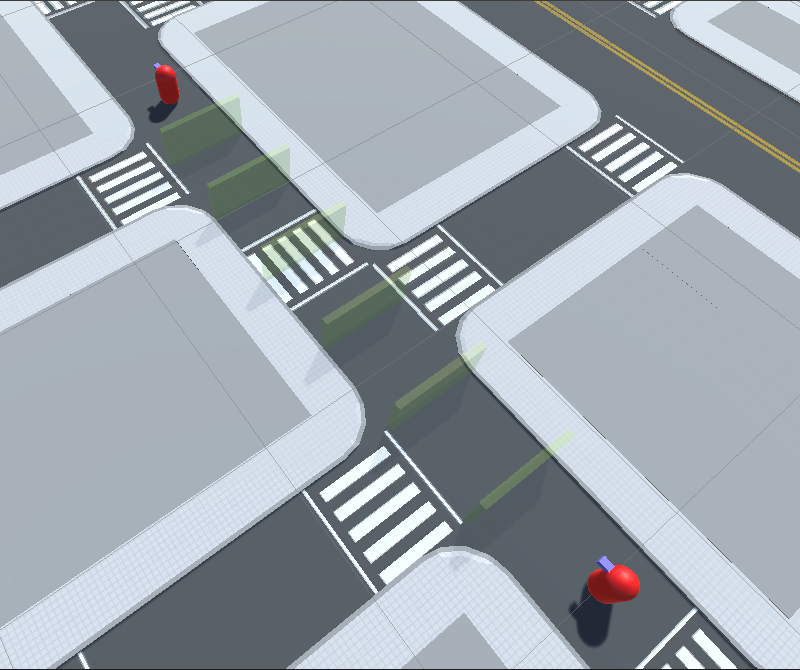
\includegraphics[scale=0.35]{figs/rotas/path_14.png}
     \caption{O percurso executado no primeiro treino. A cápsula vermelha no canto inferior direito indica a posição inicial do veículo e a na parte superior esquerdo indica o destino.}
     \label{fig:rota-1}
\end{figure}
 
\subsection*{Estatísticas}

Abaixo segue os gráficos dos dados coletados deste treino. 

\begin{figure}[h]
    \centering
    \includegraphics[scale=0.35]{figs/treinos/treino-1/política.png}
     \caption{Estatísticas referentes a política. O primeiro gráfico é a entropia, decaindo como é esperado. O terceiro gráfico é o Extrinsic Value estimate, sobe e estabiliza, conforme esperado}
     \label{fig:treino-1-politica}
\end{figure}

\begin{figure}[h]
    \centering
    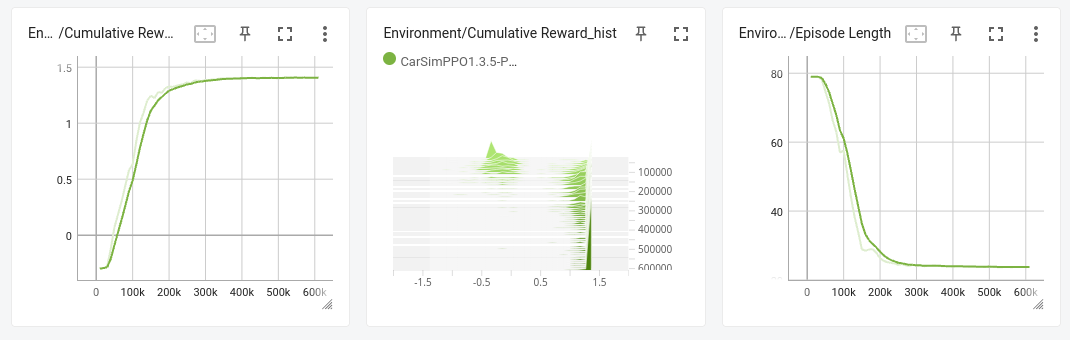
\includegraphics[scale=0.35]{figs/treinos/treino-1/ambiente.png}
     \caption{Estatísticas do ambiente. O primeiro gráfico é o acumulado de recompensa, o segundo é um histograma das distribuições de recompens. O terceiro é a duração do episódio.}
     \label{fig:treino-1-ambiente}
\end{figure}

\subsection*{Análise}
O treino foi bem sucedido, o agente soube conduzir bem o veículo. Vendo o gráfico 1 da figura 9, pode se notar o crescimento exponencial da recompensa e então sua estabilização quando atinge o máximo da recompensa que é possível receber. Também percebe-se que na mesma velocidade mas desta vez em sentido descendente a duração média do episódio, rapidamente cai pois o agente já dominou o trajeto. Isso é o suficiente para este trajeto, podemos treinar o agente em um novo desafio especifíco mas com um trajeto mais complexo.

\section{Desafio em trajeto específico dificuldade média}
Aqui o treino foi feito em dois trajetos (identificados por Path(8) e Path(0) no projeto), ambos exigem que o agente faça uma conversão do veículo.

\subsection*{Resumo}
Neste desafio foi necessário uma melhoria no agente, foi aumentado bastante o número de sensores, agora ele possui dois \textit{compenents} Ray Perception sensor 3D, o primeiro é para visão frontal e detecta os checkpoints e obstáculos e o segundo é uma visão para todas as direções do carro servindo para detecção apenas de obstáculos. Isso foi necessário pois na primeira versão havia pontos cegos, durante os testes o veículo não completava pois os sensores não detectavam o destino em sua frente.

%considerar criar um apêndice detalhando os sensores das versões do veículo
\begin{figure}[h]
    \centering
    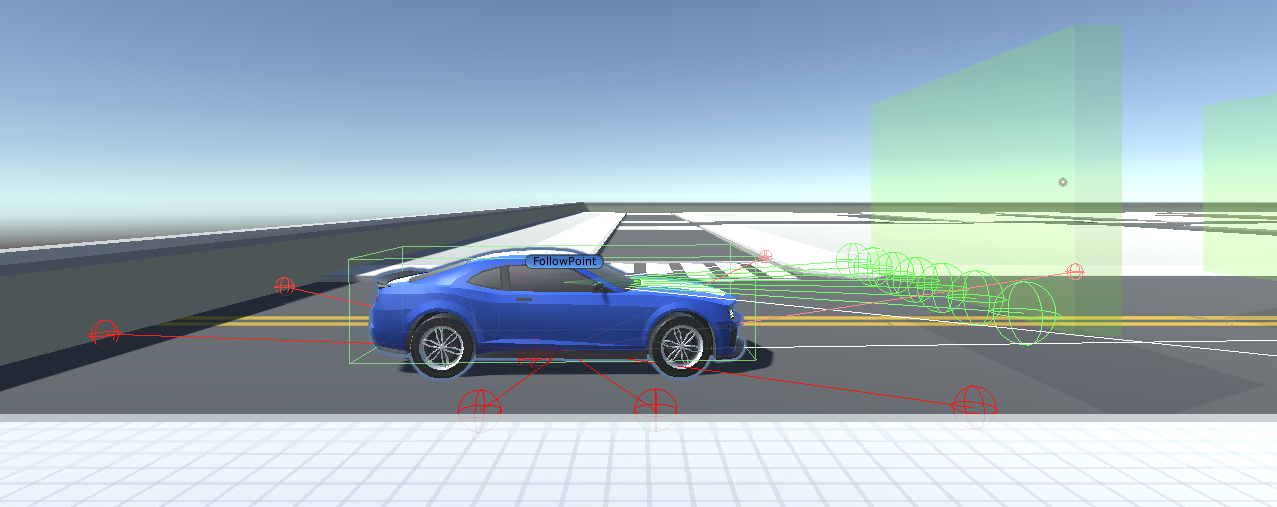
\includegraphics[scale=0.35]{figs/treinos/desafio-mediano/novo-modelo-agente.png}
     \caption{Visão lateral do novo veículo. Os superiores em verde que tem uma visão frontal, e os inferiores em vermelho que cobrem toda a volta do veículo.}
     \label{fig:desafio-2-novo-agente}
\end{figure}



\begin{table}[htpb]
    \centering
    \caption{Configuração do treino do trajeto específico de dificuldade mediana}
    \begin{tabular}{|l|p{2cm}|p{3cm}|p{3cm}|p{3.5cm}|}
         \hline
         \small{Rota(s)} & \small{Algoritmo} &          \small{params. PPO}         & \small{params. gerais} &          \small{params. RN}              \\ \hline
            Path(8)      &      PPO          &     beta: 1e-3 \newline epsilon: 0.3 &    max\_steps: 1e6  &    num\_layer:2 \newline hidden\_units:256  \\ \hline
            Path(0)      &      PPO          &     beta: 1e-3 \newline epsilon: 0.3 &    max\_steps: 1e6  &    num\_layer:2 \newline hidden\_units:256  \\ \hline
    \end{tabular}
 \end{table}

\subsection*{Estatísticas}

\begin{figure}[h]
    \centering
    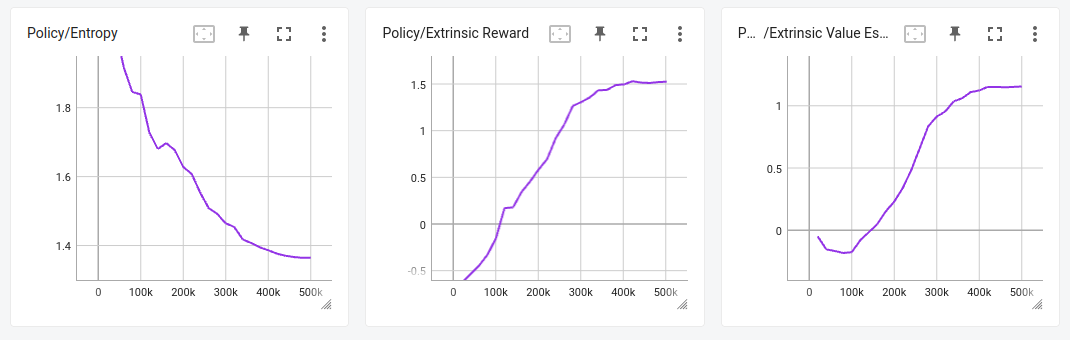
\includegraphics[scale=0.35]{figs/treinos/desafio-mediano/path0/politica.png}
    \caption{Estatísticas referentes a política do segundo desafio na rota zero.}
\end{figure}

\begin{figure}[h]
    \centering
    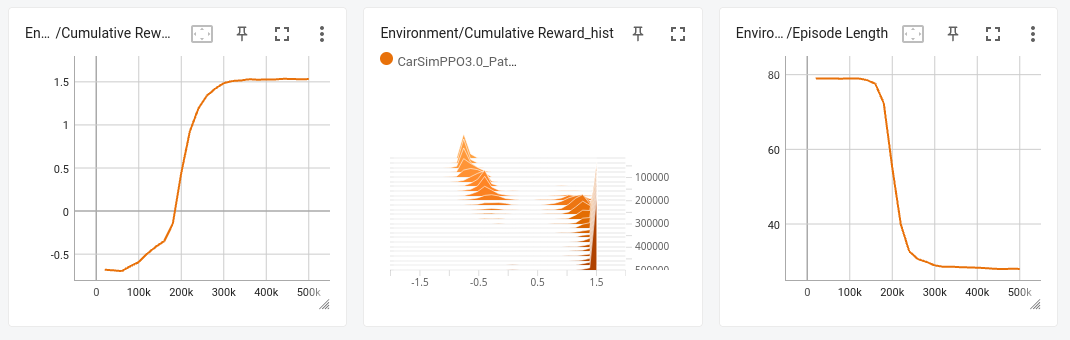
\includegraphics[scale=0.35]{figs/treinos/desafio-mediano/path0/ambiente.png}
    \caption{Estatísticas do ambiente do segundo desafio na rota zero.}
\end{figure}

\begin{figure}[h]
    \centering
    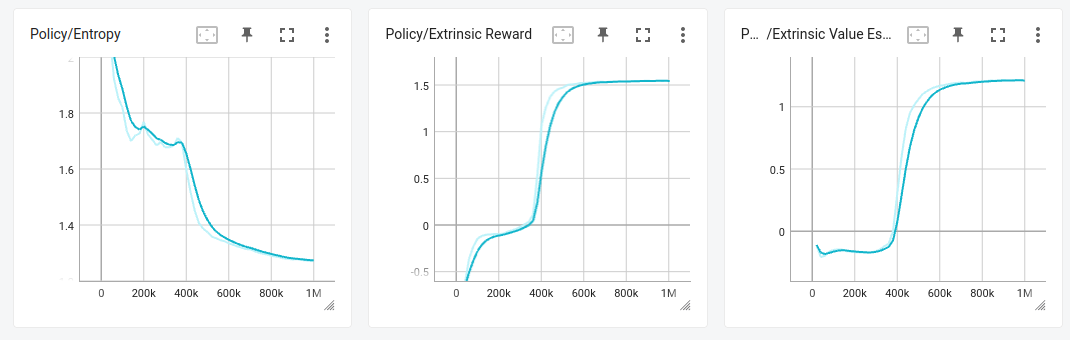
\includegraphics[scale=0.35]{figs/treinos/desafio-mediano/path8/politica.png}
    \caption{Estatísticas referentes a política do segundo desafio na rota 8.}
\end{figure}

\begin{figure}[h]
    \centering
    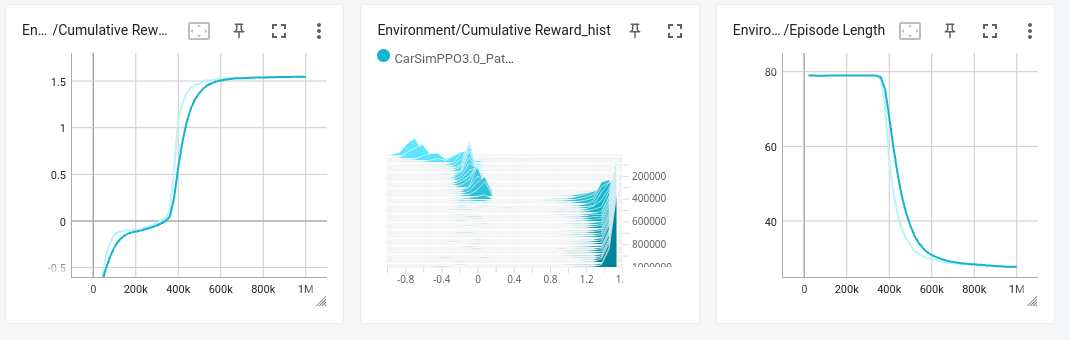
\includegraphics[scale=0.35]{figs/treinos/desafio-mediano/path8/ambiente.png}
    \caption{Estatísticas do ambiente do segundo desafio na rota 8.}
\end{figure}
\subsection*{Análise}
O modelo novo do veículo não teve problemas para 

\section{Desafio em trajeto específico difícil}
\subsection*{Resumo}
Para este desafio foi testado em três rotas diferentes, duas delas possui duas curvas e a terceira possui três curvas.

\begin{figure}[h]
    \centering
    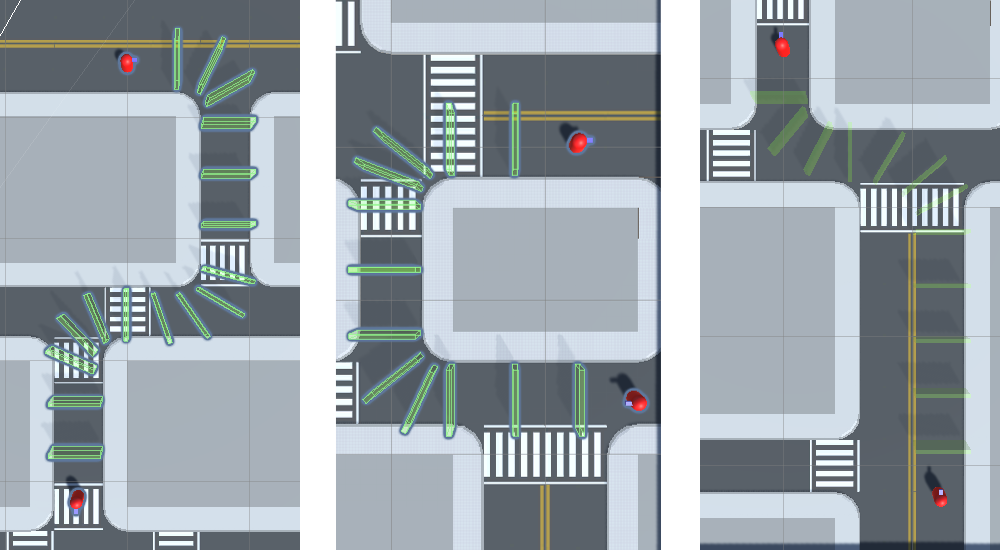
\includegraphics{figs/treinos/desafio-dificil/rotas.png}
    \caption{As três rotas difíceis envolve mais de uma curva, a esquerda o path(3) que possui três curvas sendo o mais complexo dos trajetos. Os outros dois são o path(5) e path(6) que possuem 2 curvas cada.}
\end{figure}

\begin{table}[htpb]
    \centering
    \caption{Configuração do treino do trajeto específico de dificuldade mediana}
    \begin{tabular}{|l|p{2cm}|p{3cm}|p{3cm}|p{3.5cm}|}
         \hline
         \small{Rota(s)} & \small{Algoritmo} &          \small{params. PPO}         & \small{params. gerais} &          \small{params. RN}              \\ \hline
            Path(3)      &      PPO          &     beta: 1e-3 \newline epsilon: 0.2 &    max\_steps: 2.4e6  &    num\_layer:2 \newline hidden\_units:256  \\ \hline
            Path(5)      &      PPO          &     beta: 1e-3 \newline epsilon: 0.3 &    max\_steps: 1e6  &    num\_layer:2 \newline hidden\_units:256  \\ \hline
            Path(6)      &      PPO          &     beta: 1e-3 \newline epsilon: 0.3 &    max\_steps: 1e6  &    num\_layer:2 \newline hidden\_units:256  \\ \hline
    \end{tabular}
 \end{table}

\subsection*{Estatísticas}


\subsection*{Análise}

\section{Desafio em todos os trajetos}
\subsection*{Resumo}
Por fim foi realizado o teste em todos os trajetos. Neste desafio não foi necessário qualquer alteração no agente.
\begin{table}[htpb]
    \centering
    \caption{Configuração do treino do trajeto específico de dificuldade mediana}
    \begin{tabular}{|l|p{2cm}|p{3cm}|p{3cm}|p{3.5cm}|}
         \hline
         \small{Rota(s)} & \small{Algoritmo} &          \small{params. PPO}             & \small{params. gerais} &          \small{params. RN}                  \\ \hline
            TODAS        &      PPO          &     beta: 1e-3 \newline epsilon: 0.3     &    max\_steps: 1.2e6   &    num\_layer:2 \newline hidden\_units:256   \\ \hline
    \end{tabular}
\end{table}
\subsection*{Estatísticas}
\begin{figure}[h]
    \centering
    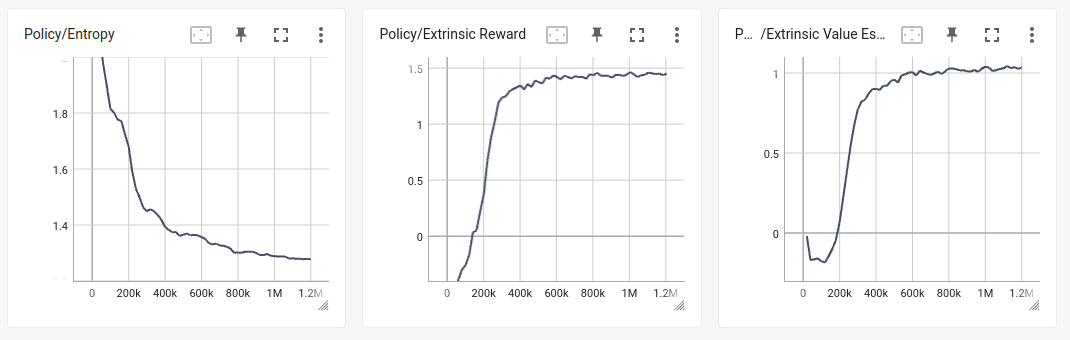
\includegraphics[scale=0.35]{figs/treinos/desafio-geral/politica.png}
    \caption{Estatísticas referentes a política do desafio geral.}
\end{figure}

\begin{figure}[h]
    \centering
    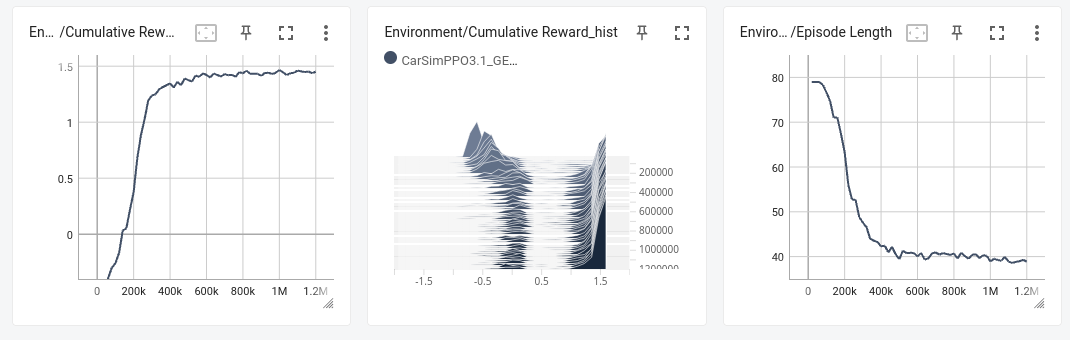
\includegraphics[scale=0.35]{figs/treinos/desafio-geral/ambiente.png}
    \caption{Estatísticas do ambiente do desafio geral.}
\end{figure}

\begin{table}[htpb]
    \centering
    \caption{Consolidado do completo do teste de todas tentativas e suas recompensas e a recompensa média por rota.}
    \label{resultado-tabela-geral}
    \begin{tabular}{|l|c|c|c|c|c|c|r|}
         \hline
         \small{Rota} & \small{C. T. 1} & \small{Rec. 1}  & \small{C. T. 2} &\small{Rec. 2} & \small{C. T. 3} &\small{Rec. 3} &\small{Rec. média}   \\ \hline
            Path(0)   &      sim        &   1             &    sim          &      1        &    sim          &      1     &      1                 \\ \hline
            Path(1)   &      sim        &   1             &    sim          &      1        &    sim          &      1     &      1                 \\ \hline
            Path(2)   &      sim        &   1             &    sim          &      1        &    sim          &      1     &      1                 \\ \hline
            Path(3)   &      não        &   -0.18         &    sim          &      0.85     &    sim          &      1     &      0.56              \\ \hline
            Path(4)   &      sim        &   1             &    sim          &      1        &    sim          &      1     &      1                 \\ \hline
            Path(5)   &      sim        &   1             &    sim          &      0.8      &    sim          &      1     &      0.93              \\ \hline
            Path(6)   &      sim        &   1             &    não          &      -0.31    &    sim          &      1     &      0.56              \\ \hline
            Path(7)   &      sim        &   0.85          &    sim          &      1        &    sim          &      0.9   &      0.91              \\ \hline
            Path(8)   &      sim        &   1             &    sim          &      0.9      &    sim          &      1     &      0.96              \\ \hline
            Path(9)   &      sim        &   1             &    sim          &      0.95     &    sim          &      1     &      0.98              \\ \hline
            Path(10)  &      não        &   0.12          &    não          &      0.02     &    sim          &      1     &      0.38              \\ \hline
            Path(11)  &      sim        &   1             &    sim          &      1        &    sim          &      1     &      1                 \\ \hline
            Path(12)  &      sim        &   1             &    sim          &      1        &    sim          &      1     &      1                 \\ \hline
            Path(13)  &      sim        &   1             &    sim          &      1        &    sim          &      1     &      1                 \\ \hline
            Path(14)  &      sim        &   1             &    sim          &      1        &    sim          &      1     &      1                 \\ \hline
            Path(15)  &      sim        &   1             &    sim          &      1        &    sim          &      1     &      1                 \\ \hline
            Path(16)  &      sim        &   1             &    sim          &      1        &    sim          &      1     &      1                 \\ \hline
    \end{tabular}
\end{table}
\subsection*{Análise}
O desafio foi um sucesso, o treino utilizando de PPO convergiu por volta dos 600 mil passos, metade do limite, o agente "percebeu" rapidamente que seu objetivo era atingir cada checkpoint até o destino. O teste no geral foi positivo sendo perfeito em 10 dos 17 trajetos, obtendo 0,89 de média geral e concluindo 48 dos 51 tentativas. 
Porém se fizermos um recorte de trajetos difíceis (duas ou mais curvas) teremos um resultado não tão satisfatório. Neste caso seriam além dos envolvidos no desafio anterior, seriam os Path's de número 7, 10, 12 e 14, teríamos 18 conclusões de 21 corridas feitas (85\%), todas as vezes que o agente falhou foram em um desses e com média de apenas 0,63 de recompensa.